% This file was created by tikzplotlib vunknown.
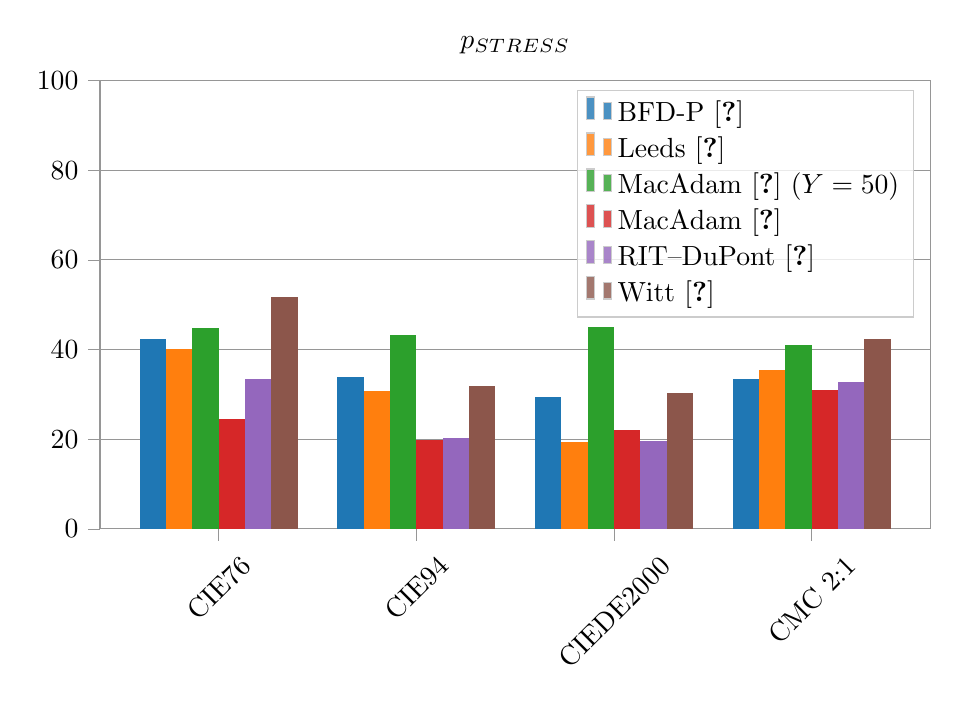
\begin{tikzpicture}

\definecolor{color0}{rgb}{0.12156862745098,0.466666666666667,0.705882352941177}
\definecolor{color1}{rgb}{1,0.498039215686275,0.0549019607843137}
\definecolor{color2}{rgb}{0.172549019607843,0.627450980392157,0.172549019607843}
\definecolor{color3}{rgb}{0.83921568627451,0.152941176470588,0.156862745098039}
\definecolor{color4}{rgb}{0.580392156862745,0.403921568627451,0.741176470588235}
\definecolor{color5}{rgb}{0.549019607843137,0.337254901960784,0.294117647058824}

\begin{axis}[
axis line style={white!58.8235294117647!black},
height=0.6\textwidth,
legend cell align={left},
legend style={fill opacity=0.8, draw opacity=1, text opacity=1, draw=white!80!black},
tick align=outside,
tick pos=left,
title={\(\displaystyle p_{STRESS}\)},
width=\textwidth,
x grid style={white!58.8235294117647!black},
xmin=-0.6, xmax=3.6,
xtick style={color=white!58.8235294117647!black},
xtick={0,1,2,3},
xticklabel style = {rotate=45.0},
xticklabels={CIE76,CIE94,CIEDE2000,CMC 2:1},
y grid style={white!58.8235294117647!black},
ymajorgrids,
ymin=0, ymax=100,
ytick style={color=white!58.8235294117647!black}
]
\draw[draw=none,fill=color0] (axis cs:-0.4,0) rectangle (axis cs:-0.266666666666667,42.4095489785527);
\addlegendimage{ybar,ybar legend,draw=none,fill=color0};
\addlegendentry{BFD-P \cite{luorigg}}

\draw[draw=none,fill=color0] (axis cs:0.6,0) rectangle (axis cs:0.733333333333333,33.9166220461603);
\draw[draw=none,fill=color0] (axis cs:1.6,0) rectangle (axis cs:1.73333333333333,29.5212723042391);
\draw[draw=none,fill=color0] (axis cs:2.6,0) rectangle (axis cs:2.73333333333333,33.506587074841);
\draw[draw=none,fill=color1] (axis cs:-0.266666666666667,0) rectangle (axis cs:-0.133333333333333,40.0364176602205);
\addlegendimage{ybar,ybar legend,draw=none,fill=color1};
\addlegendentry{Leeds \cite{leeds}}

\draw[draw=none,fill=color1] (axis cs:0.733333333333333,0) rectangle (axis cs:0.866666666666667,30.7398552375823);
\draw[draw=none,fill=color1] (axis cs:1.73333333333333,0) rectangle (axis cs:1.86666666666667,19.4609191829183);
\draw[draw=none,fill=color1] (axis cs:2.73333333333333,0) rectangle (axis cs:2.86666666666667,35.4800406903705);
\draw[draw=none,fill=color2] (axis cs:-0.133333333333333,0) rectangle (axis cs:2.77555756156289e-17,44.8952155515788);
\addlegendimage{ybar,ybar legend,draw=none,fill=color2};
\addlegendentry{MacAdam \cite{macadam1942} ($Y=50$)}

\draw[draw=none,fill=color2] (axis cs:0.866666666666667,0) rectangle (axis cs:1,43.1638593810694);
\draw[draw=none,fill=color2] (axis cs:1.86666666666667,0) rectangle (axis cs:2,45.0506021909445);
\draw[draw=none,fill=color2] (axis cs:2.86666666666667,0) rectangle (axis cs:3,41.1259051595414);
\draw[draw=none,fill=color3] (axis cs:4.16333634234434e-17,0) rectangle (axis cs:0.133333333333333,24.5319191673876);
\addlegendimage{ybar,ybar legend,draw=none,fill=color3};
\addlegendentry{MacAdam \cite{macadam1974}}

\draw[draw=none,fill=color3] (axis cs:1,0) rectangle (axis cs:1.13333333333333,19.7853974310146);
\draw[draw=none,fill=color3] (axis cs:2,0) rectangle (axis cs:2.13333333333333,22.1289373697461);
\draw[draw=none,fill=color3] (axis cs:3,0) rectangle (axis cs:3.13333333333333,30.9828303427505);
\draw[draw=none,fill=color4] (axis cs:0.133333333333333,0) rectangle (axis cs:0.266666666666667,33.364735317963);
\addlegendimage{ybar,ybar legend,draw=none,fill=color4};
\addlegendentry{RIT--DuPont \cite{berns}}

\draw[draw=none,fill=color4] (axis cs:1.13333333333333,0) rectangle (axis cs:1.26666666666667,20.3557004987779);
\draw[draw=none,fill=color4] (axis cs:2.13333333333333,0) rectangle (axis cs:2.26666666666667,19.5111243169988);
\draw[draw=none,fill=color4] (axis cs:3.13333333333333,0) rectangle (axis cs:3.26666666666667,32.8046660031734);
\draw[draw=none,fill=color5] (axis cs:0.266666666666667,0) rectangle (axis cs:0.4,51.6740349454926);
\addlegendimage{ybar,ybar legend,draw=none,fill=color5};
\addlegendentry{Witt \cite{witt}}

\draw[draw=none,fill=color5] (axis cs:1.26666666666667,0) rectangle (axis cs:1.4,31.9666655304065);
\draw[draw=none,fill=color5] (axis cs:2.26666666666667,0) rectangle (axis cs:2.4,30.369462501181);
\draw[draw=none,fill=color5] (axis cs:3.26666666666667,0) rectangle (axis cs:3.4,42.3944471199168);
\end{axis}

\end{tikzpicture}
